\begin{figure}[th!]
\begin{center}
\begin{small}
\begin{sc}
\begin{tabular}{c@{\hskip2pt}c@{\hskip2pt}c@{\hskip2pt}c@{\hskip2pt}c}
Input&Ours&AME&GlAtEx&AttSeg\\
% 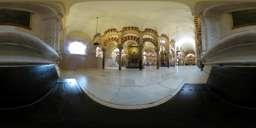
\includegraphics[width=\smallimg]{figures/rec_sun/1/gt.jpg}&
\includegraphics[width=\smallimg]{figures/rec_sun/1/ours.png}&\includegraphics[width=\smallimg]
% {figures/rec_sun/1/ame.jpg}&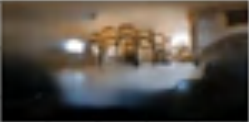
\includegraphics[width=\smallimg]{figures/rec_sun/1/glatex.png}&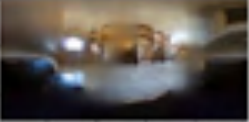
\includegraphics[width=\smallimg]{figures/rec_sun/1/atseg.png}\\

\includegraphics[width=\smallimg]{figures/rec_sun/2/gt.jpg}&
\includegraphics[width=\smallimg]
{figures/rec_sun/2/ours.png}&
\includegraphics[width=\smallimg]
{figures/rec_sun/2/ame.jpg}&
\includegraphics[width=\smallimg]{figures/rec_sun/2/glatex.png}&
\includegraphics[width=\smallimg]{figures/rec_sun/2/atseg.png}\\

\includegraphics[width=\smallimg]{figures/rec_sun/3/gt.jpg}&
\includegraphics[width=\smallimg]{figures/rec_sun/3/ours.png}&
\includegraphics[width=\smallimg]
{figures/rec_sun/3/ame.jpg}&
\includegraphics[width=\smallimg]{figures/rec_sun/3/glatex.png}&
\includegraphics[width=\smallimg]{figures/rec_sun/3/atseg.png}\\
% 
\includegraphics[width=\smallimg]{figures/rec_sun/4/gt.jpg}&
\includegraphics[width=\smallimg]{figures/rec_sun/4/ours.png}&\includegraphics[width=\smallimg]
% {figures/rec_sun/4/ame.jpg}&
\includegraphics[width=\smallimg]{figures/rec_sun/4/glatex.png}&
\includegraphics[width=\smallimg]{figures/rec_sun/4/atseg.png}\\
\end{tabular}
\begin{tabular}{c@{\hskip2pt}c@{\hskip2pt}c@{\hskip2pt}c|c@{\hskip2pt}c@{\hskip2pt}c@{\hskip2pt}c}
Input&Ours&AME&SimGlim&Input&Ours&AME&SimGlim\\

\includegraphics[width=\smallerimg]{figures/rec_ade/3/gt.jpg}&
\includegraphics[width=\smallerimg]{figures/rec_ade/3/ours.png}&
\includegraphics[width=\smallerimg]{figures/rec_ade/3/ame.jpg}&
\includegraphics[width=\smallerimg]{figures/rec_ade/3/simglim.png}&

\includegraphics[width=\smallerimg]{figures/rec_ade/2/gt.jpg}&
\includegraphics[width=\smallerimg]{figures/rec_ade/2/ours.png}&
\includegraphics[width=\smallerimg]{figures/rec_ade/2/ame.jpg}&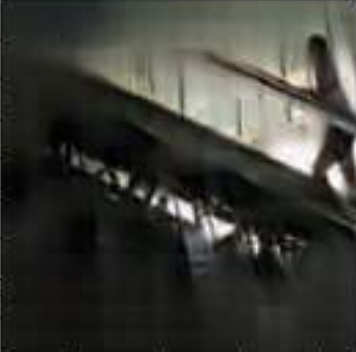
\includegraphics[width=\smallerimg]{figures/rec_ade/2/simglim.png}\\

\includegraphics[width=\smallerimg]{figures/rec_ade/4/gt.jpg}&
\includegraphics[width=\smallerimg]{figures/rec_ade/4/ours.png}&
\includegraphics[width=\smallerimg]{figures/rec_ade/4/ame.jpg}&
\includegraphics[width=\smallerimg]{figures/rec_ade/4/simglim.png}&

\includegraphics[width=\smallerimg]{figures/rec_ade/1/gt.jpg}&
\includegraphics[width=\smallerimg]{figures/rec_ade/1/ours.png}&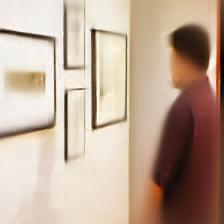
\includegraphics[width=\smallerimg]{figures/rec_ade/1/ame.jpg}&
\includegraphics[width=\smallerimg]{figures/rec_ade/1/simglim.png}\\
\end{tabular}
\end{sc}
\end{small}
\end{center}
\vspace{-.2cm}
\caption{\textbf{Reconstruction quality for SUN360 (top) and ADE20K (bottom):} Sample reconstructions of our method compared with AME \cite{pardyl2023active}, AttSeg~\protect\cite{seifi2020attend}, GlAtEx~\protect\cite{seifi2021glimpse} and SimGlim~\protect\cite{jha2023simglim} on the SUN360 and ADE20K datasets. Reconstructions done with our method are visibly more detailed and less blurry than those obtained by baseline methods. Notice that images for comparison were taken from the baseline publications (we did not select them).}
\label{fig:qualiative}
\end{figure}